% Options for packages loaded elsewhere
\PassOptionsToPackage{unicode}{hyperref}
\PassOptionsToPackage{hyphens}{url}
\PassOptionsToPackage{dvipsnames,svgnames,x11names}{xcolor}
%
\documentclass[
  letterpaper,
  DIV=11,
  numbers=noendperiod]{scrartcl}

\usepackage{amsmath,amssymb}
\usepackage{iftex}
\ifPDFTeX
  \usepackage[T1]{fontenc}
  \usepackage[utf8]{inputenc}
  \usepackage{textcomp} % provide euro and other symbols
\else % if luatex or xetex
  \usepackage{unicode-math}
  \defaultfontfeatures{Scale=MatchLowercase}
  \defaultfontfeatures[\rmfamily]{Ligatures=TeX,Scale=1}
\fi
\usepackage{lmodern}
\ifPDFTeX\else  
    % xetex/luatex font selection
\fi
% Use upquote if available, for straight quotes in verbatim environments
\IfFileExists{upquote.sty}{\usepackage{upquote}}{}
\IfFileExists{microtype.sty}{% use microtype if available
  \usepackage[]{microtype}
  \UseMicrotypeSet[protrusion]{basicmath} % disable protrusion for tt fonts
}{}
\makeatletter
\@ifundefined{KOMAClassName}{% if non-KOMA class
  \IfFileExists{parskip.sty}{%
    \usepackage{parskip}
  }{% else
    \setlength{\parindent}{0pt}
    \setlength{\parskip}{6pt plus 2pt minus 1pt}}
}{% if KOMA class
  \KOMAoptions{parskip=half}}
\makeatother
\usepackage{xcolor}
\usepackage[top=0.75in,bottom=0.75in,left=0.75in,right=0.75in]{geometry}
\setlength{\emergencystretch}{3em} % prevent overfull lines
\setcounter{secnumdepth}{-\maxdimen} % remove section numbering
% Make \paragraph and \subparagraph free-standing
\makeatletter
\ifx\paragraph\undefined\else
  \let\oldparagraph\paragraph
  \renewcommand{\paragraph}{
    \@ifstar
      \xxxParagraphStar
      \xxxParagraphNoStar
  }
  \newcommand{\xxxParagraphStar}[1]{\oldparagraph*{#1}\mbox{}}
  \newcommand{\xxxParagraphNoStar}[1]{\oldparagraph{#1}\mbox{}}
\fi
\ifx\subparagraph\undefined\else
  \let\oldsubparagraph\subparagraph
  \renewcommand{\subparagraph}{
    \@ifstar
      \xxxSubParagraphStar
      \xxxSubParagraphNoStar
  }
  \newcommand{\xxxSubParagraphStar}[1]{\oldsubparagraph*{#1}\mbox{}}
  \newcommand{\xxxSubParagraphNoStar}[1]{\oldsubparagraph{#1}\mbox{}}
\fi
\makeatother


\providecommand{\tightlist}{%
  \setlength{\itemsep}{0pt}\setlength{\parskip}{0pt}}\usepackage{longtable,booktabs,array}
\usepackage{calc} % for calculating minipage widths
% Correct order of tables after \paragraph or \subparagraph
\usepackage{etoolbox}
\makeatletter
\patchcmd\longtable{\par}{\if@noskipsec\mbox{}\fi\par}{}{}
\makeatother
% Allow footnotes in longtable head/foot
\IfFileExists{footnotehyper.sty}{\usepackage{footnotehyper}}{\usepackage{footnote}}
\makesavenoteenv{longtable}
\usepackage{graphicx}
\makeatletter
\def\maxwidth{\ifdim\Gin@nat@width>\linewidth\linewidth\else\Gin@nat@width\fi}
\def\maxheight{\ifdim\Gin@nat@height>\textheight\textheight\else\Gin@nat@height\fi}
\makeatother
% Scale images if necessary, so that they will not overflow the page
% margins by default, and it is still possible to overwrite the defaults
% using explicit options in \includegraphics[width, height, ...]{}
\setkeys{Gin}{width=\maxwidth,height=\maxheight,keepaspectratio}
% Set default figure placement to htbp
\makeatletter
\def\fps@figure{htbp}
\makeatother

\usepackage{booktabs}
\usepackage{longtable}
\usepackage{array}
\usepackage{multirow}
\usepackage{wrapfig}
\usepackage{float}
\usepackage{colortbl}
\usepackage{pdflscape}
\usepackage{tabu}
\usepackage{threeparttable}
\usepackage{threeparttablex}
\usepackage[normalem]{ulem}
\usepackage{makecell}
\usepackage{xcolor}
\usepackage{caption}
\usepackage{anyfontsize}
\usepackage{fancyhdr}
\pagestyle{empty}
\thispagestyle{empty}
\KOMAoption{captions}{tableheading}
\makeatletter
\@ifpackageloaded{caption}{}{\usepackage{caption}}
\AtBeginDocument{%
\ifdefined\contentsname
  \renewcommand*\contentsname{Table of contents}
\else
  \newcommand\contentsname{Table of contents}
\fi
\ifdefined\listfigurename
  \renewcommand*\listfigurename{List of Figures}
\else
  \newcommand\listfigurename{List of Figures}
\fi
\ifdefined\listtablename
  \renewcommand*\listtablename{List of Tables}
\else
  \newcommand\listtablename{List of Tables}
\fi
\ifdefined\figurename
  \renewcommand*\figurename{Figure}
\else
  \newcommand\figurename{Figure}
\fi
\ifdefined\tablename
  \renewcommand*\tablename{Table}
\else
  \newcommand\tablename{Table}
\fi
}
\@ifpackageloaded{float}{}{\usepackage{float}}
\floatstyle{ruled}
\@ifundefined{c@chapter}{\newfloat{codelisting}{h}{lop}}{\newfloat{codelisting}{h}{lop}[chapter]}
\floatname{codelisting}{Listing}
\newcommand*\listoflistings{\listof{codelisting}{List of Listings}}
\makeatother
\makeatletter
\makeatother
\makeatletter
\@ifpackageloaded{caption}{}{\usepackage{caption}}
\@ifpackageloaded{subcaption}{}{\usepackage{subcaption}}
\makeatother

\ifLuaTeX
  \usepackage{selnolig}  % disable illegal ligatures
\fi
\usepackage{bookmark}

\IfFileExists{xurl.sty}{\usepackage{xurl}}{} % add URL line breaks if available
\urlstyle{same} % disable monospaced font for URLs
\hypersetup{
  pdftitle={California Sentinel Sites for Nature (CA-SSN) Gap Analysis},
  colorlinks=true,
  linkcolor={blue},
  filecolor={Maroon},
  citecolor={Blue},
  urlcolor={Blue},
  pdfcreator={LaTeX via pandoc}}


\title{California Sentinel Sites for Nature (CA-SSN) Gap Analysis}
\author{}
\date{}

\begin{document}
\maketitle


\section{Introduction}\label{introduction}

\textbf{About the Sentinel Site Network (SSN)}

The California Sentinel Site Network (SSN) is a set of standardized
biodiversity and climate monitoring sites. Four partners manage sites
across the state: UCNRS, CDFW, TNC, and Pepperwood. Each site follows
common field methods so we can compare trends across regions and
partners.

\textbf{Why use EPA ecoregions}

EPA ecoregions group places with similar climate, soils, hydrology,
landforms, and potential vegetation. The system is hierarchical: Level I
represents continental patterns (broad realms); Level II shows
sub-continental regions; Level III indicates major ecological regions
within states (useful for statewide planning); and Level IV captures
local subsections with finer variation (useful for site-level coverage).

For a California gap analysis, Level III shows which major ecological
regions our network reaches, while Level IV shows which local
subsections we cover or miss. We map both to see broad representation
(L3) and fine-scale coverage (L4).

\section{CA-SSN Sites and US EPA Level III
Ecoregions}\label{ca-ssn-sites-and-us-epa-level-iii-ecoregions}

\begin{figure}[H]

{\centering 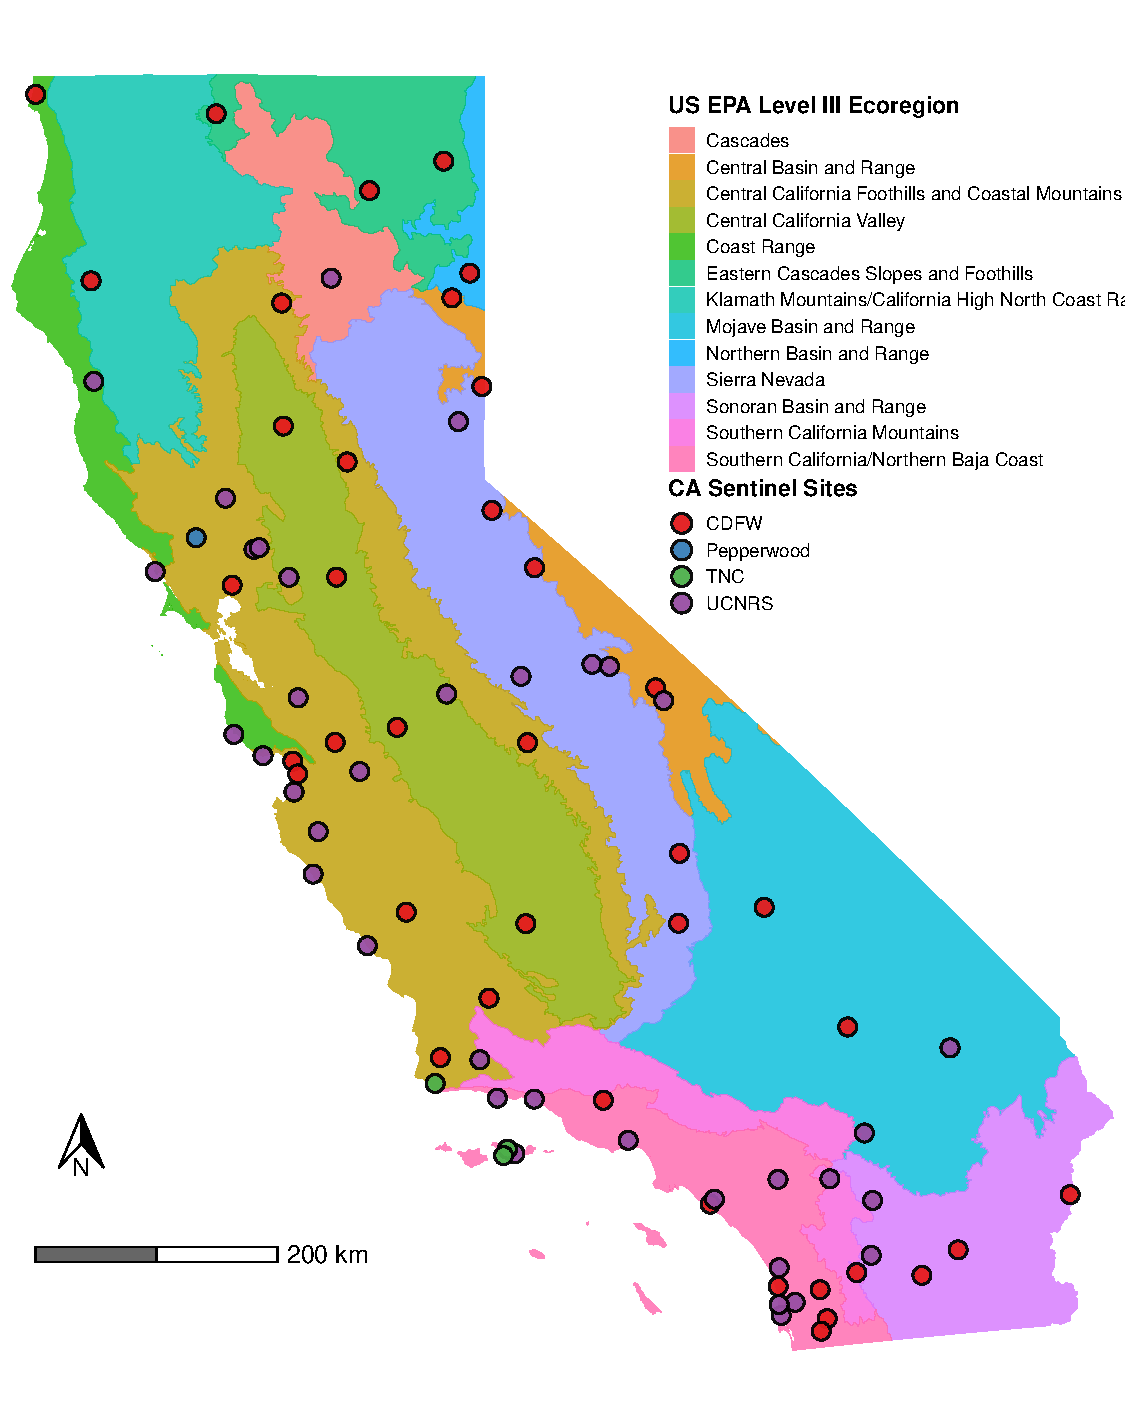
\includegraphics[width=1\textwidth,height=\textheight]{01_analyze_files/figure-pdf/map-L3-SSN-1.pdf}

}

\caption{California Sentinel Sites for Nature (CA-SSN) monitoring sites
across 13 US EPA Level III ecoregions. Sites are shown by managing
organization (CDFW, Pepperwood Preserve, TNC, UCNRS) and all 13 Level
III ecoregions are covered by at least one sentinel site.}

\end{figure}%

\begingroup\fontsize{9}{11}\selectfont

\begin{longtable}[t]{>{\raggedright\arraybackslash}p{3.5cm}>{\raggedleft\arraybackslash}p{1cm}>{\raggedright\arraybackslash}p{10cm}}
\caption{Level III Ecoregion Coverage: 13 of 13 ecoregions covered by Sentinel Sites}\\
\toprule
\textbf{Level III Ecoregion} & \textbf{Sites} & \textbf{Sentinel Sites}\\
\midrule
\endfirsthead
\caption[]{Level III Ecoregion Coverage: 13 of 13 ecoregions covered by Sentinel Sites \textit{(continued)}}\\
\toprule
\textbf{Level III Ecoregion} & \textbf{Sites} & \textbf{Sentinel Sites}\\
\midrule
\endhead

\endfoot
\bottomrule
\endlastfoot
\cellcolor{gray!10}{Cascades} & \cellcolor{gray!10}{1} & \cellcolor{gray!10}{Lassen Field Station (UCNRS)}\\
Central Basin and Range & 5 & Fish Slough Ecological Reserve (CDFW); Hallelujah Junction Wildlife Area (CDFW); Honey Lake Wildlife Area (CDFW); Sierra Nevada Aquatic Research Lab (UCNRS); White Mountain Research Center (UCNRS)\\
\cellcolor{gray!10}{Central California Foothills and Coastal Mountains} & \cellcolor{gray!10}{23} & \cellcolor{gray!10}{Big Sandy Wildlife Area (CDFW); Big Table Mountain Ecological Reserve (CDFW); Blue Oak Ranch Reserve (UCNRS); Burton Mesa Ecological Reserve (CDFW); Cañada de Los Osos Ecological Reserve (CDFW); Carrizo Plains Ecological Reserve (CDFW); Dangermond @ Jalama HQ (TNC); Elkhorn Slough Ecological Reserve (CDFW); Fort Ord (UCNRS); Hastings Natural Reservation (UCNRS); Ken Norris Rancho Marino Reserve (UCNRS); Landels Hill Big Creek Reserve (UCNRS); McLaughlin Reserve (UCNRS); Napa-Sonoma Marshes Wildlife Area (CDFW); Pepperwood Preserve (Pepperwood); Quail Ridge Reserve (UCNRS); Sedgwick Reserve (UCNRS); Spenceville Wildlife Area (CDFW); Stebbins Cold Canyon Reserve (UCNRS); Strathearn (UCNRS); Tehama Wildlife Area (CDFW); Watsonville Slough Ecological Reserve (CDFW); Younger Lagoon (UCNRS)}\\
Central California Valley & 6 & Cosumnes River Ecological Reserve (CDFW); Jepson Praire Reserve (UCNRS); Merced Vernal Pools (UCNRS); North Grasslands Wildlife Area (CDFW); Semitropic Ecological Reserve (CDFW); Upper Butte Basin Wildlife Area (CDFW)\\
\cellcolor{gray!10}{Coast Range} & \cellcolor{gray!10}{3} & \cellcolor{gray!10}{Angelo Reserve (UCNRS); Bodega Marine Lab and Reserve (UCNRS); Lake Earl Wildlife Area (CDFW)}\\
\addlinespace
Eastern Cascades Slopes and Foothills & 3 & Ash Creek Wildlife Area (CDFW); Fitzhugh Creek Wildlife Area (CDFW); Shasta Valley Wildlife Area (CDFW)\\
\cellcolor{gray!10}{Klamath Mountains/California High North Coast Range} & \cellcolor{gray!10}{1} & \cellcolor{gray!10}{McLellan Mountain Peatland (CDFW)}\\
Mojave Basin and Range & 4 & Burns Piñon Ridge Reserve (UCNRS); Camp Cady Wildlife Area (CDFW); Granites Desert Research Station (UCNRS); Indian Joe Springs Ecological Reserve (CDFW)\\
\cellcolor{gray!10}{Northern Basin and Range} & \cellcolor{gray!10}{1} & \cellcolor{gray!10}{Great Basin Springs (Five Springs) (CDFW)}\\
Sierra Nevada & 7 & Canebrake Ecological Reserve (CDFW); Hope Valley Wildlife Area (CDFW); Monache Meadows Wildlife Area (CDFW); Pickel Meadow Wildlife Area (CDFW); Sagehen Creek Field Station (UCNRS); Valentine Reserve (UCNRS); Yosemite Field Station (UCNRS)\\
\addlinespace
\cellcolor{gray!10}{Sonoran Basin and Range} & \cellcolor{gray!10}{6} & \cellcolor{gray!10}{Anza Borrego (UCNRS); Boyd Deep Canyon Reserve (UCNRS); Imperial Wildlife Area (CDFW); Palo Verde Ecological Reserve (CDFW); San Felipe Creek Ecological Reserve (CDFW); San Felipe Valley Wildlife Area (CDFW)}\\
Southern California Mountains & 1 & James Reserve (UCNRS)\\
\cellcolor{gray!10}{Southern California/Northern Baja Coast} & \cellcolor{gray!10}{17} & \cellcolor{gray!10}{Canada de San Vicente Ecological Reserve (CDFW); Carpinteria Marsh Reserve (UCNRS); Cienega Springs Ecological Reserve (CDFW); Coal Oil Point Reserve (UCNRS); Dawson Reserve (UCNRS); Elliot Chaparral Reserve (UCNRS); Motte Rimrock Reserve (UCNRS); Rancho Jamul Ecological Reserve (CDFW); San Elijo Lagoon Ecological Reserve (CDFW); San Joaquin Marsh Reserve (UCNRS); Santa Cruz Island @ Diablo Peak (TNC); Santa Cruz Island @ Sierra Blanca (TNC); Santa Cruz Island Reserve (UCNRS); Scripps Coastal Reserve (UCNRS); Stunt Ranch Reserve (UCNRS); Sycuan Peak Ecological Reserve (CDFW); Upper Newport Bay Ecological Reserve (CDFW)}\\*
\end{longtable}
\endgroup{}

\section{CA-SSN Sites and Level IV
Ecoregions}\label{ca-ssn-sites-and-level-iv-ecoregions}

\begin{figure}[H]

{\centering 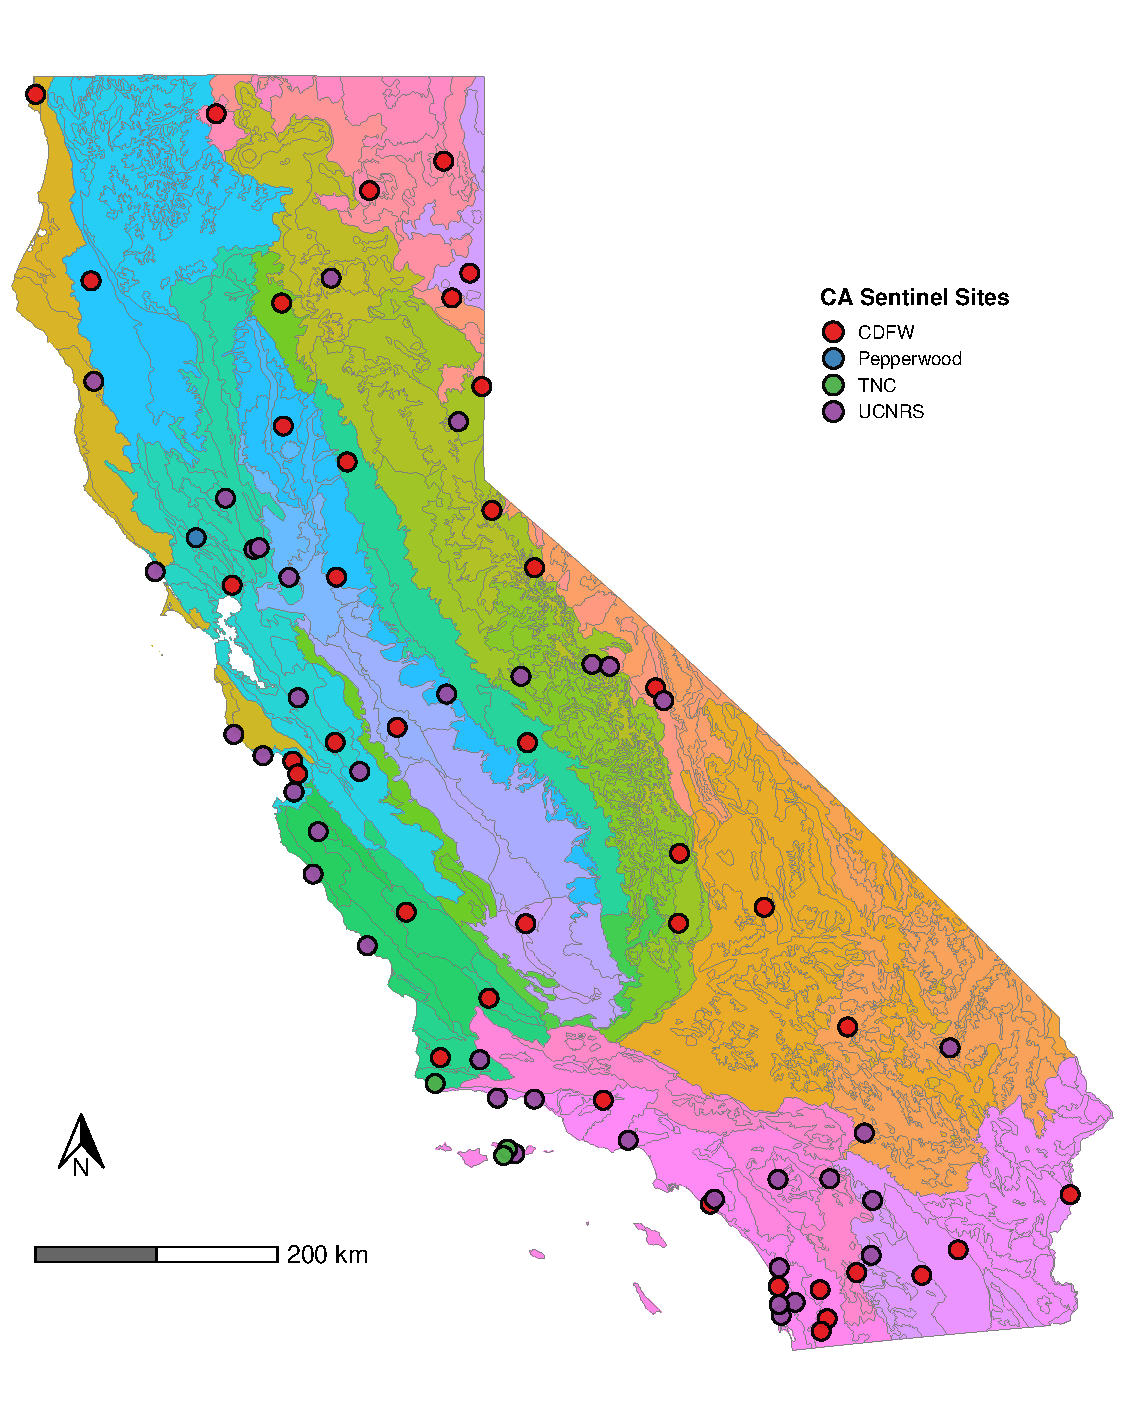
\includegraphics[width=1\textwidth,height=\textheight]{01_analyze_files/figure-pdf/map-L4-SSN-1.pdf}

}

\caption{California Sentinel Site Network (CA-SSN) monitoring sites by
managing organization across 180 US EPA Level IV ecoregions. Level IV
ecoregions provide finer ecological classification than Level III. See
following pages for complete Level IV ecoregion legend.}

\end{figure}%

\begin{figure}[H]

{\centering 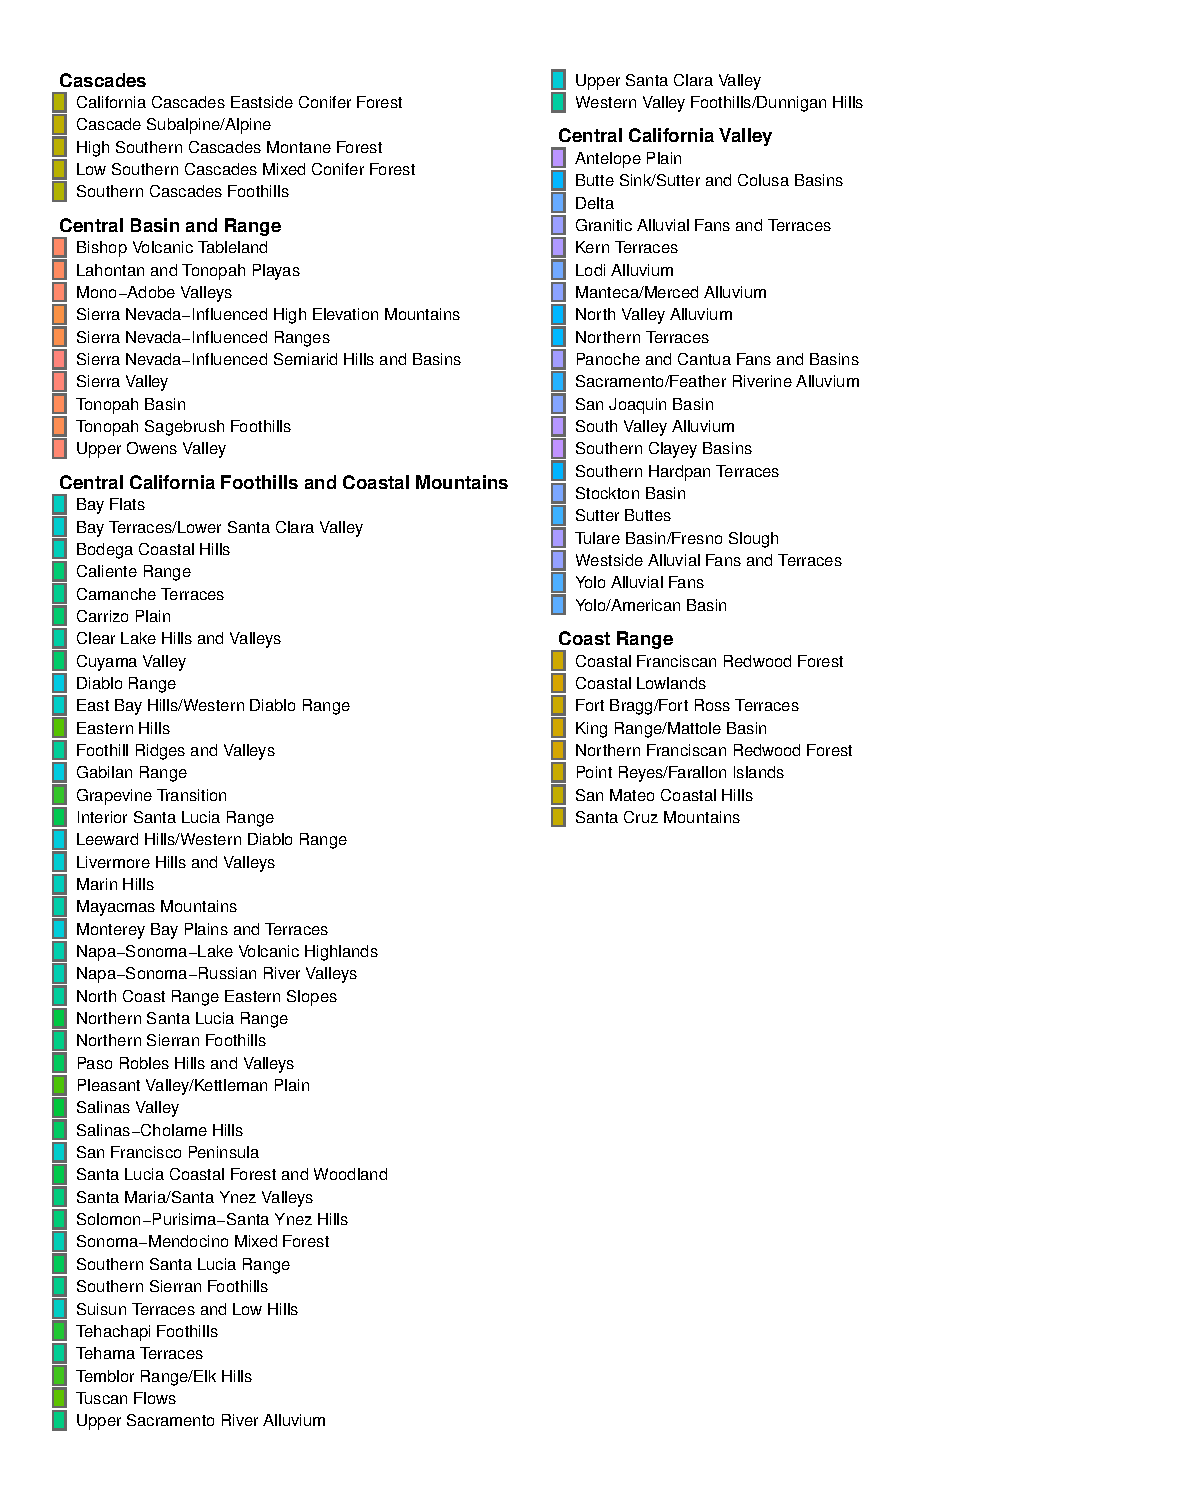
\includegraphics[width=1\textwidth,height=\textheight]{01_analyze_files/figure-pdf/legend-L4-page1-1.pdf}

}

\caption{Legend for US EPA Level IV ecoregions in California (Part 1 of
2), organized by Level III ecoregion.}

\end{figure}%

\newpage

\begin{figure}[H]

{\centering 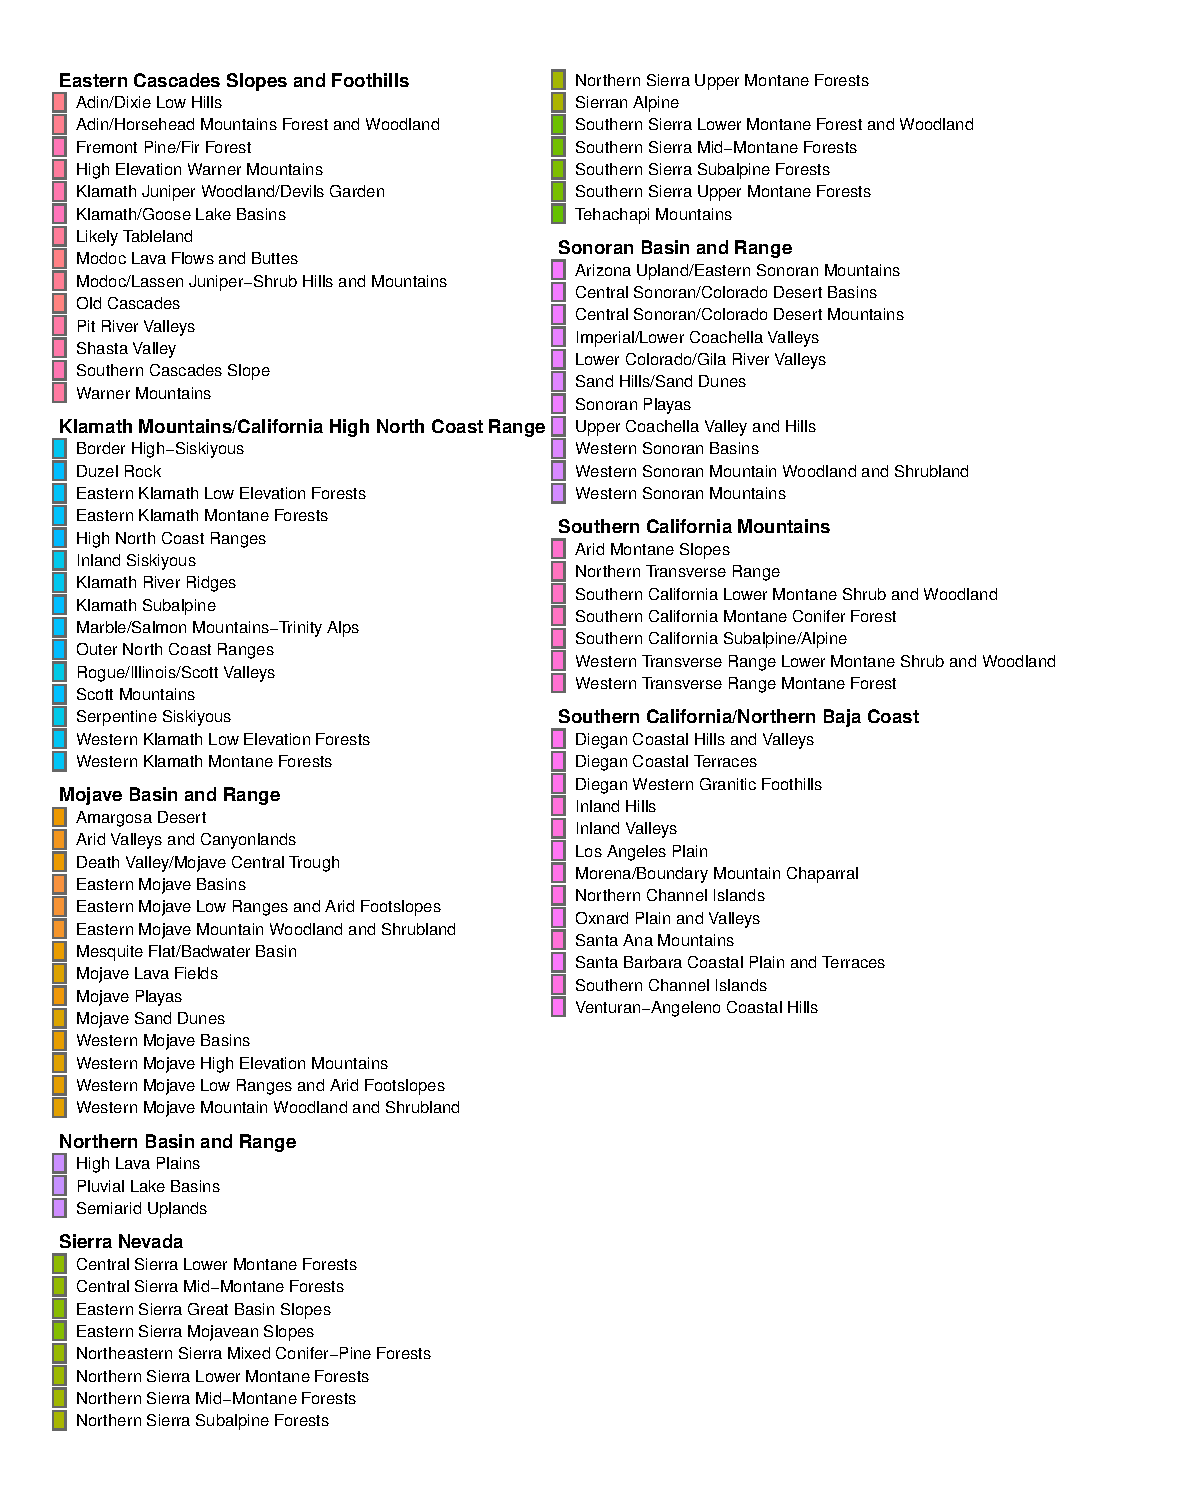
\includegraphics[width=1\textwidth,height=\textheight]{01_analyze_files/figure-pdf/legend-L4-page2-1.pdf}

}

\caption{Legend for US EPA Level IV ecoregions in California (Part 2 of
2), organized by Level III ecoregion.}

\end{figure}%

\newpage

\section{Explore Coverage and Identify
Gaps}\label{explore-coverage-and-identify-gaps}

\begin{table}
\caption*{
{\fontsize{20}{25}\selectfont  \textbf{Sentinel Site coverage across US EPA ecoregions}\fontsize{12}{15}\selectfont } \\ 
{\fontsize{14}{17}\selectfont  Counts of Level III and IV ecoregions represented by at least one Sentinel Site\fontsize{12}{15}\selectfont }
} 
\fontsize{12.0pt}{14.0pt}\selectfont
\begin{tabular*}{\linewidth}{@{\extracolsep{\fill}}>{\centering\arraybackslash}p{\dimexpr 180.00pt -2\tabcolsep-1.5\arrayrulewidth}>{\centering\arraybackslash}p{\dimexpr 105.00pt -2\tabcolsep-1.5\arrayrulewidth}>{\centering\arraybackslash}p{\dimexpr 120.00pt -2\tabcolsep-1.5\arrayrulewidth}}
\toprule
Metric & Coverage & Missing ecoregions \\ 
\midrule\addlinespace[2.5pt]
Level III ecoregions & 13 of 13 & 0 \\ 
Level IV ecoregions & 56 of 180 & 124 \\ 
\bottomrule
\end{tabular*}
\end{table}

\begin{verbatim}
Scale on map varies by more than 10%, scale bar may be inaccurate
Scale on map varies by more than 10%, scale bar may be inaccurate
\end{verbatim}

\begin{figure}[H]

{\centering 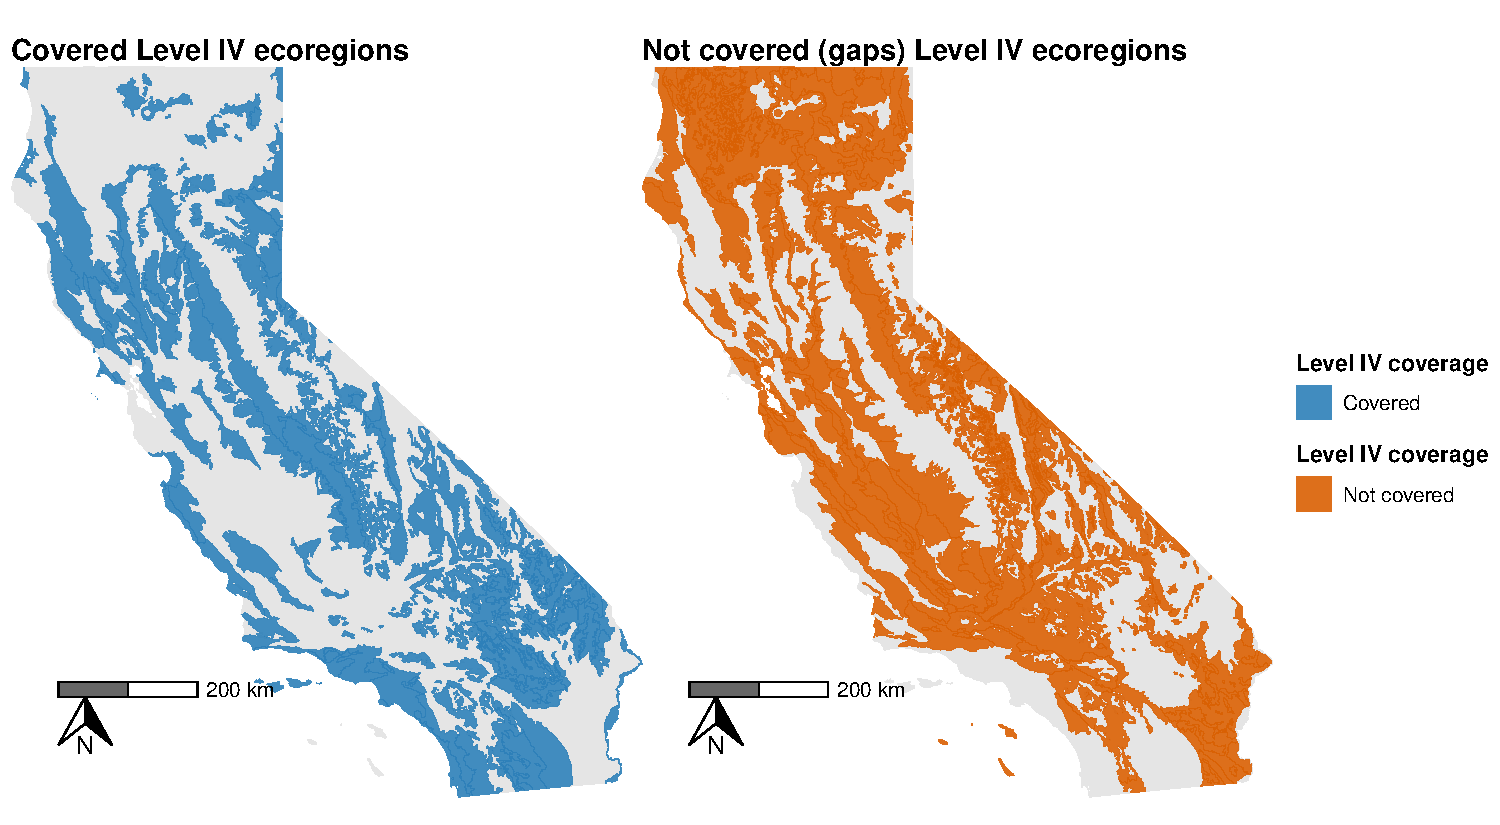
\includegraphics[width=1\textwidth,height=\textheight]{01_analyze_files/figure-pdf/coverage-maps-1.pdf}

}

\caption{Spatial distribution of Level IV ecoregion coverage by CA-SSN
sites. Left: ecoregions with at least one site (blue). Right: ecoregions
without sites (orange).}

\end{figure}%

\newpage

\begin{table}
\caption*{
{\fontsize{20}{25}\selectfont  \textbf{Level IV Ecoregion Coverage}\fontsize{12}{15}\selectfont } \\ 
{\fontsize{14}{17}\selectfont  \textbf{Covered:} 56 / 180 (31.1\%)  •  \textbf{Not covered:} 124 / 180 (68.9\%)\fontsize{12}{15}\selectfont }
} 
\fontsize{12.0pt}{14.0pt}\selectfont
\begin{tabular*}{1\linewidth}{@{\extracolsep{\fill}}>{\raggedright\arraybackslash}p{\dimexpr 390.00pt -2\tabcolsep-1.5\arrayrulewidth}>{\raggedright\arraybackslash}p{\dimexpr 390.00pt -2\tabcolsep-1.5\arrayrulewidth}}
\toprule
Level IV ecoregions \textemdash Covered & Level IV ecoregions \textemdash Not covered \\ 
\midrule\addlinespace[2.5pt]
Bishop Volcanic Tableland & Adin/Dixie Low Hills \\ 
Butte Sink/Sutter and Colusa Basins & Adin/Horsehead Mountains Forest and Woodland \\ 
Caliente Range & Amargosa Desert \\ 
Coastal Franciscan Redwood Forest & Antelope Plain \\ 
Coastal Lowlands & Arid Montane Slopes \\ 
Diegan Coastal Hills and Valleys & Arid Valleys and Canyonlands \\ 
Diegan Coastal Terraces & Arizona Upland/Eastern Sonoran Mountains \\ 
Diegan Western Granitic Foothills & Bay Flats \\ 
East Bay Hills/Western Diablo Range & Bay Terraces/Lower Santa Clara Valley \\ 
Eastern Mojave Basins & Bodega Coastal Hills \\ 
Eastern Mojave Low Ranges and Arid Footslopes & Border High-Siskiyous \\ 
Eastern Sierra Great Basin Slopes & California Cascades Eastside Conifer Forest \\ 
Foothill Ridges and Valleys & Camanche Terraces \\ 
High Lava Plains & Carrizo Plain \\ 
High Southern Cascades Montane Forest & Cascade Subalpine/Alpine \\ 
Imperial/Lower Coachella Valleys & Central Sierra Lower Montane Forests \\ 
Inland Hills & Central Sierra Mid-Montane Forests \\ 
Likely Tableland & Central Sonoran/Colorado Desert Basins \\ 
Los Angeles Plain & Central Sonoran/Colorado Desert Mountains \\ 
Lower Colorado/Gila River Valleys & Clear Lake Hills and Valleys \\ 
Mayacmas Mountains & Cuyama Valley \\ 
Monterey Bay Plains and Terraces & Death Valley/Mojave Central Trough \\ 
Napa-Sonoma-Russian River Valleys & Delta \\ 
North Coast Range Eastern Slopes & Diablo Range \\ 
Northeastern Sierra Mixed Conifer-Pine Forests & Duzel Rock \\ 
Northern Channel Islands & Eastern Hills \\ 
Northern Santa Lucia Range & Eastern Klamath Low Elevation Forests \\ 
Northern Sierra Upper Montane Forests & Eastern Klamath Montane Forests \\ 
Northern Sierran Foothills & Eastern Mojave Mountain Woodland and Shrubland \\ 
Northern Terraces & Eastern Sierra Mojavean Slopes \\ 
Outer North Coast Ranges & Fort Bragg/Fort Ross Terraces \\ 
Oxnard Plain and Valleys & Fremont Pine/Fir Forest \\ 
Paso Robles Hills and Valleys & Gabilan Range \\ 
Pit River Valleys & Granitic Alluvial Fans and Terraces \\ 
Point Reyes/Farallon Islands & Grapevine Transition \\ 
San Joaquin Basin & High Elevation Warner Mountains \\ 
Santa Barbara Coastal Plain and Terraces & High North Coast Ranges \\ 
Santa Lucia Coastal Forest and Woodland & Inland Siskiyous \\ 
Shasta Valley & Inland Valleys \\ 
Sierra Nevada-Influenced Semiarid Hills and Basins & Interior Santa Lucia Range \\ 
Solomon-Purisima-Santa Ynez Hills & Kern Terraces \\ 
Southern California Montane Conifer Forest & King Range/Mattole Basin \\ 
Southern Clayey Basins & Klamath Juniper Woodland/Devils Garden \\ 
Southern Hardpan Terraces & Klamath River Ridges \\ 
Southern Santa Lucia Range & Klamath Subalpine \\ 
Southern Sierra Lower Montane Forest and Woodland & Klamath/Goose Lake Basins \\ 
Southern Sierra Upper Montane Forests & Lahontan and Tonopah Playas \\ 
Southern Sierran Foothills & Leeward Hills/Western Diablo Range \\ 
Tuscan Flows & Livermore Hills and Valleys \\ 
Upper Owens Valley & Lodi Alluvium \\ 
Venturan-Angeleno Coastal Hills & Low Southern Cascades Mixed Conifer Forest \\ 
Western Mojave Low Ranges and Arid Footslopes & Manteca/Merced Alluvium \\ 
Western Sonoran Basins & Marble/Salmon Mountains-Trinity Alps \\ 
Western Sonoran Mountain Woodland and Shrubland & Marin Hills \\ 
Western Sonoran Mountains & Mesquite Flat/Badwater Basin \\ 
Yolo Alluvial Fans & Modoc Lava Flows and Buttes \\ 
 & Modoc/Lassen Juniper-Shrub Hills and Mountains \\ 
 & Mojave Lava Fields \\ 
 & Mojave Playas \\ 
 & Mojave Sand Dunes \\ 
 & Mono-Adobe Valleys \\ 
 & Morena/Boundary Mountain Chaparral \\ 
 & Napa-Sonoma-Lake Volcanic Highlands \\ 
 & North Valley Alluvium \\ 
 & Northern Franciscan Redwood Forest \\ 
 & Northern Sierra Lower Montane Forests \\ 
 & Northern Sierra Mid-Montane Forests \\ 
 & Northern Sierra Subalpine Forests \\ 
 & Northern Transverse Range \\ 
 & Old Cascades \\ 
 & Panoche and Cantua Fans and Basins \\ 
 & Pleasant Valley/Kettleman Plain \\ 
 & Pluvial Lake Basins \\ 
 & Rogue/Illinois/Scott Valleys \\ 
 & Sacramento/Feather Riverine Alluvium \\ 
 & Salinas Valley \\ 
 & Salinas-Cholame Hills \\ 
 & San Francisco Peninsula \\ 
 & San Mateo Coastal Hills \\ 
 & Sand Hills/Sand Dunes \\ 
 & Santa Ana Mountains \\ 
 & Santa Cruz Mountains \\ 
 & Santa Maria/Santa Ynez Valleys \\ 
 & Scott Mountains \\ 
 & Semiarid Uplands \\ 
 & Serpentine Siskiyous \\ 
 & Sierra Nevada-Influenced High Elevation Mountains \\ 
 & Sierra Nevada-Influenced Ranges \\ 
 & Sierra Valley \\ 
 & Sierran Alpine \\ 
 & Sonoma-Mendocino Mixed Forest \\ 
 & Sonoran Playas \\ 
 & South Valley Alluvium \\ 
 & Southern California Lower Montane Shrub and Woodland \\ 
 & Southern California Subalpine/Alpine \\ 
 & Southern Cascades Foothills \\ 
 & Southern Cascades Slope \\ 
 & Southern Channel Islands \\ 
 & Southern Sierra Mid-Montane Forests \\ 
 & Southern Sierra Subalpine Forests \\ 
 & Stockton Basin \\ 
 & Suisun Terraces and Low Hills \\ 
 & Sutter Buttes \\ 
 & Tehachapi Foothills \\ 
 & Tehachapi Mountains \\ 
 & Tehama Terraces \\ 
 & Temblor Range/Elk Hills \\ 
 & Tonopah Basin \\ 
 & Tonopah Sagebrush Foothills \\ 
 & Tulare Basin/Fresno Slough \\ 
 & Upper Coachella Valley and Hills \\ 
 & Upper Sacramento River Alluvium \\ 
 & Upper Santa Clara Valley \\ 
 & Warner Mountains \\ 
 & Western Klamath Low Elevation Forests \\ 
 & Western Klamath Montane Forests \\ 
 & Western Mojave Basins \\ 
 & Western Mojave High Elevation Mountains \\ 
 & Western Mojave Mountain Woodland and Shrubland \\ 
 & Western Transverse Range Lower Montane Shrub and Woodland \\ 
 & Western Transverse Range Montane Forest \\ 
 & Western Valley Foothills/Dunnigan Hills \\ 
 & Westside Alluvial Fans and Terraces \\ 
 & Yolo/American Basin \\ 
\bottomrule
\end{tabular*}
\end{table}




\end{document}
